\section{Membrane Potential Initialization}
\label{sec:first_method}

TCS~\cite{bntt:2020, tebn:2022, tab:2024} limits the performance of SNNs during inference, particularly when batch normalization (BN) is employed. Despite BN's capability to normalize activations during training, the fixed normalization statistics during inference result in activation drift across timesteps, causing accuracy degradation. Previous methods~\cite{tebn:2022, tab:2024} have tried to address this issue through timestep-dependent normalization, but these approaches remain superficial as they fail to resolve the underlying cause: drift in the membrane potential of LIF neurons.

To tackle this issue, we propose \textbf{MP-Init (Membrane Potential Initialization)}, an efficient solution that directly targets TCS in the membrane potential. MP-Init ensures stable activation distributions throughout inference by initializing the membrane potential of spiking neurons in each layer to match their stationary distribution. This eliminates the need for timestep-dependent normalization and enhances final performance by aligning training and inference statistics.

\begin{figure}[t!]
  \centering
  \begin{subfigure}{0.495\linewidth}
    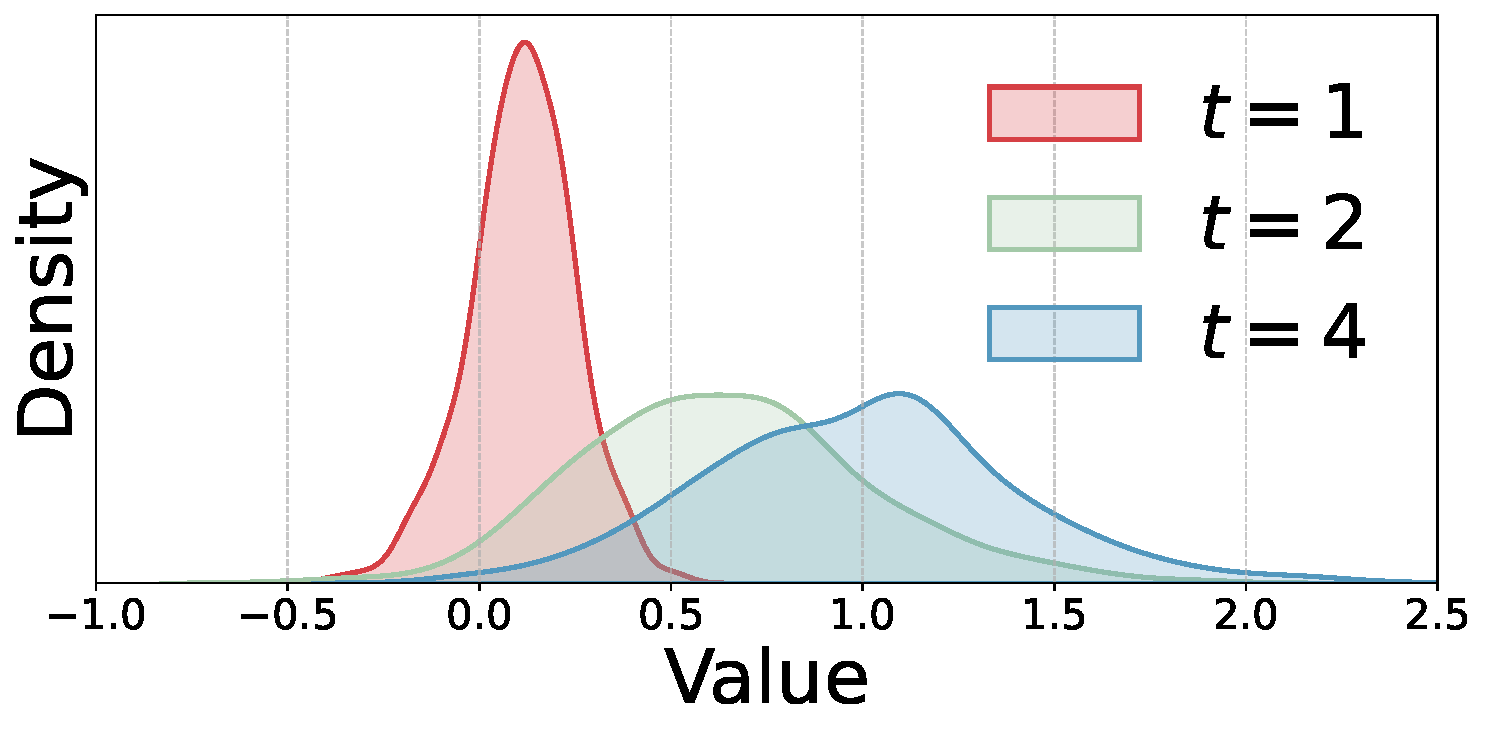
\includegraphics[width=0.95\linewidth]{fig/density_plot_membrane_potential_tdbn.pdf}
    \caption{tdBN}
    \label{fig:membrane_potential_a}
  \end{subfigure}
  \hfill
  \begin{subfigure}{0.495\linewidth}
    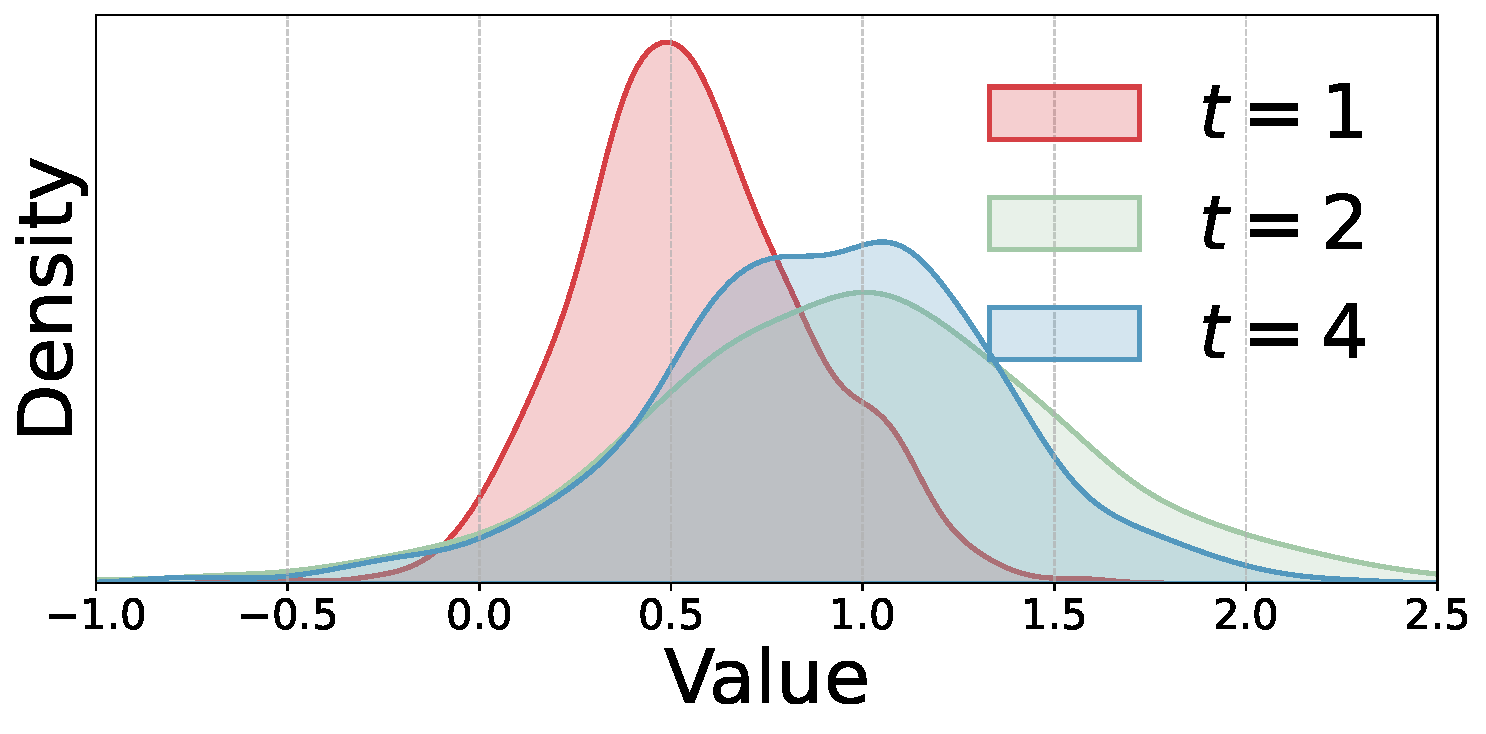
\includegraphics[width=0.95\linewidth]{fig/density_plot_membrane_potential_tebn.pdf}
    \caption{TEBN}
  \end{subfigure}
  \begin{subfigure}{0.495\linewidth}
    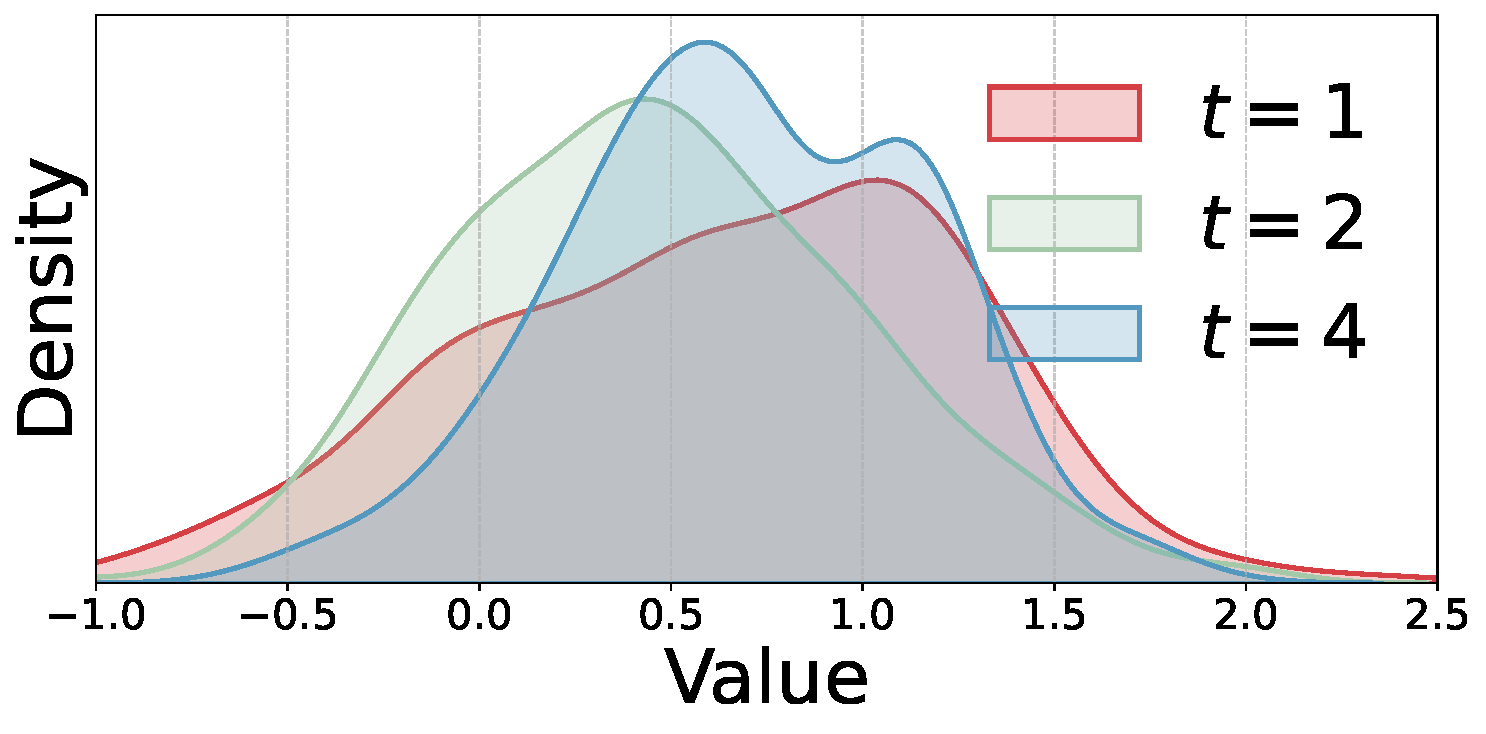
\includegraphics[width=0.95\linewidth]{fig/density_plot_membrane_potential_tab.pdf}
    \caption{TAB}
  \end{subfigure}
  \hfill
  \begin{subfigure}{0.495\linewidth}
    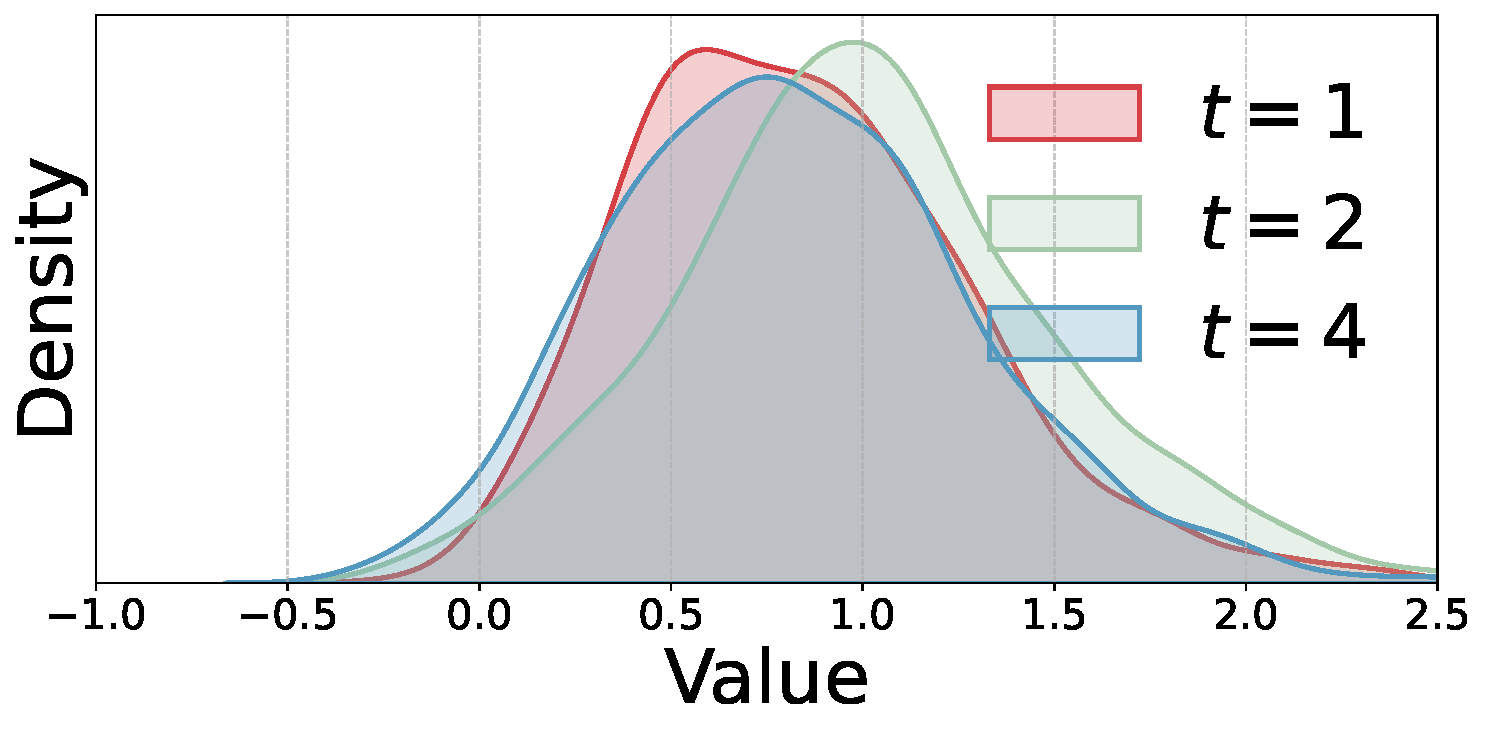
\includegraphics[width=0.95\linewidth]{fig/density_plot_membrane_potential_mpinit.pdf}
    \caption{MP-Init}
  \end{subfigure}
  \caption{Membrane potential distribution of the third layer's first spiking layer of ResNet-19 on CIFAR100}
  \label{fig:combined_membrane}
\end{figure}

\begin{figure}[t!]
  \centering
  \begin{subfigure}{0.495\linewidth}
    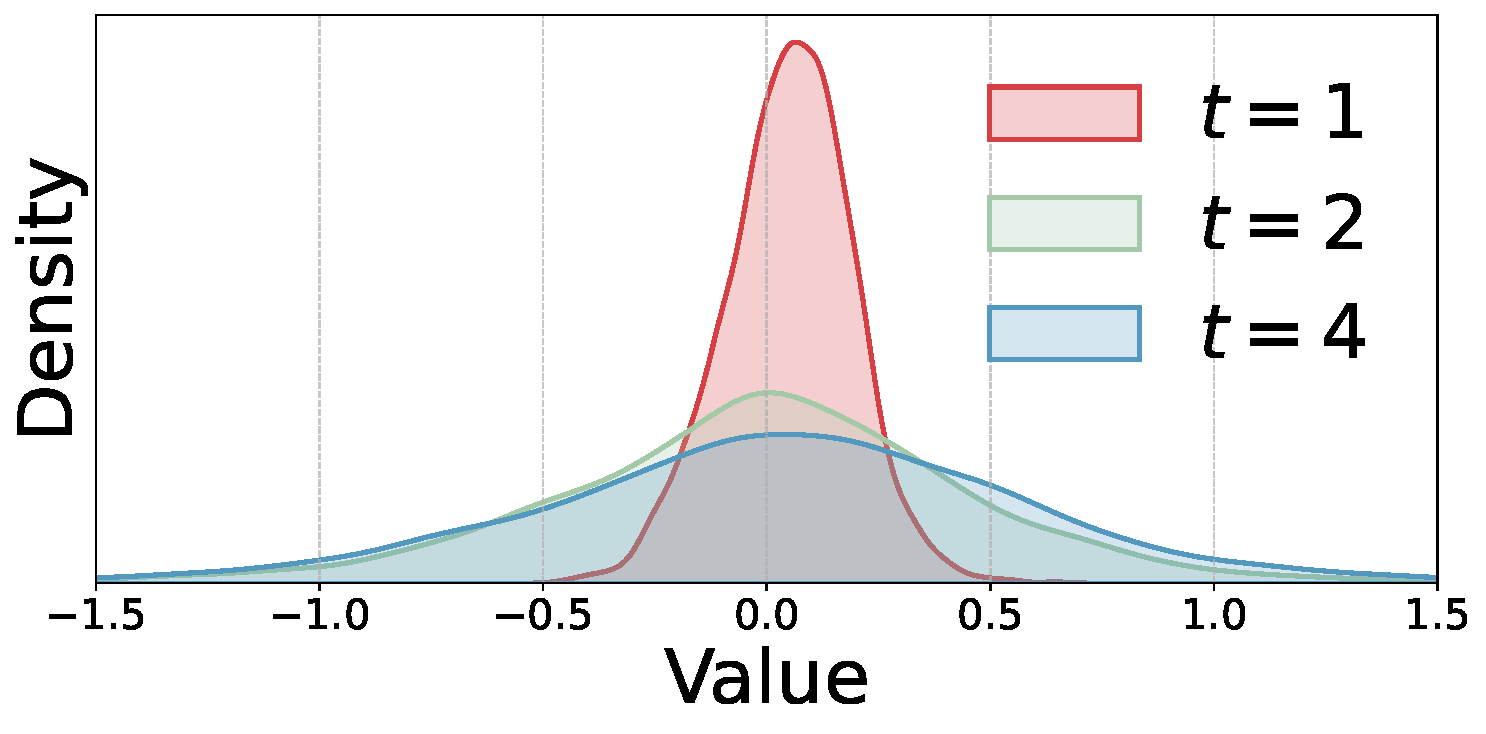
\includegraphics[width=0.95\linewidth]{fig/density_plot_presynaptic_input_tdbn.pdf}
    \caption{tdBN}
    \label{fig:presynaptic_input_a}
  \end{subfigure}
  \hfill
  \begin{subfigure}{0.495\linewidth}
    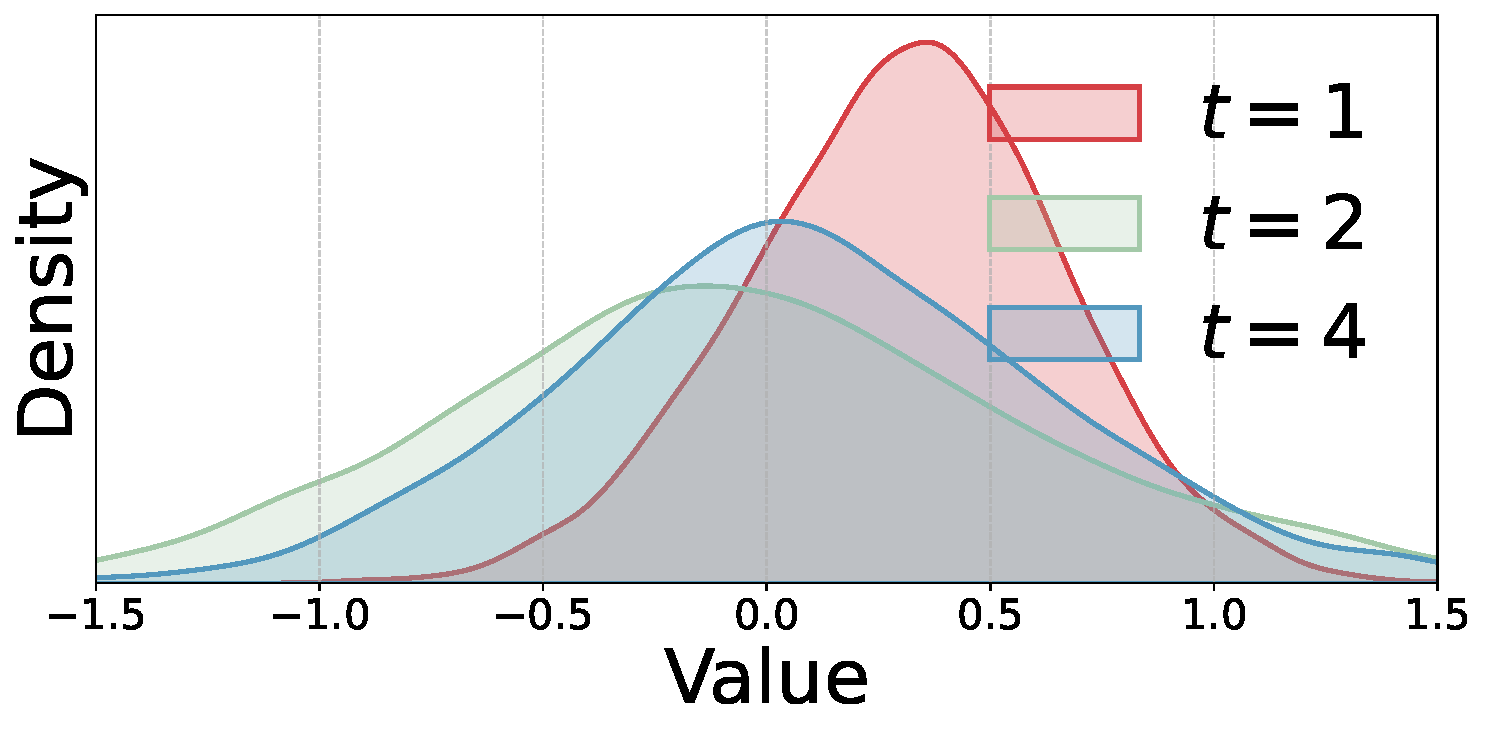
\includegraphics[width=0.95\linewidth]{fig/density_plot_presynaptic_input_tebn.pdf}
    \caption{TEBN}
  \end{subfigure}
  \begin{subfigure}{0.495\linewidth}
    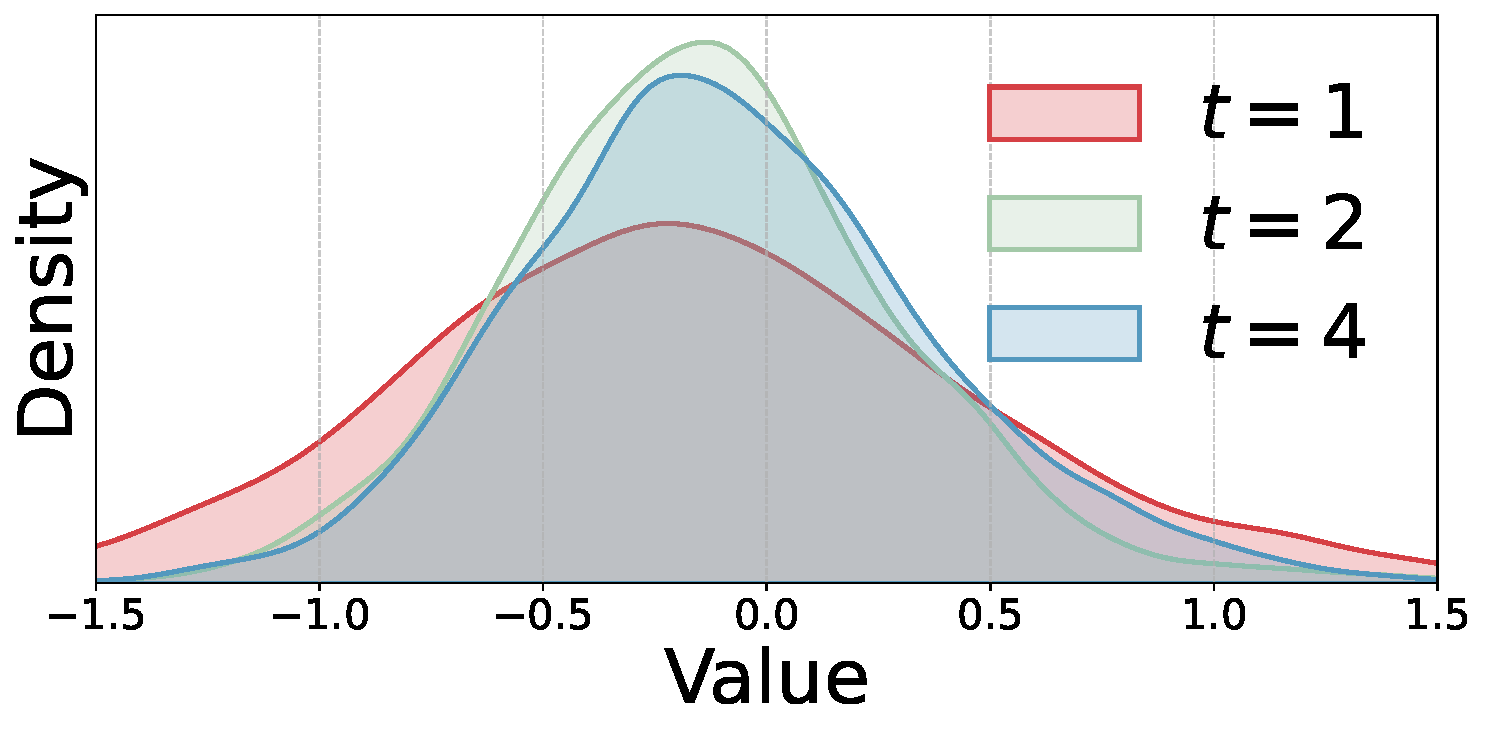
\includegraphics[width=0.95\linewidth]{fig/density_plot_presynaptic_input_tab.pdf}
    \caption{TAB}
  \end{subfigure}
  \hfill
  \begin{subfigure}{0.495\linewidth}
    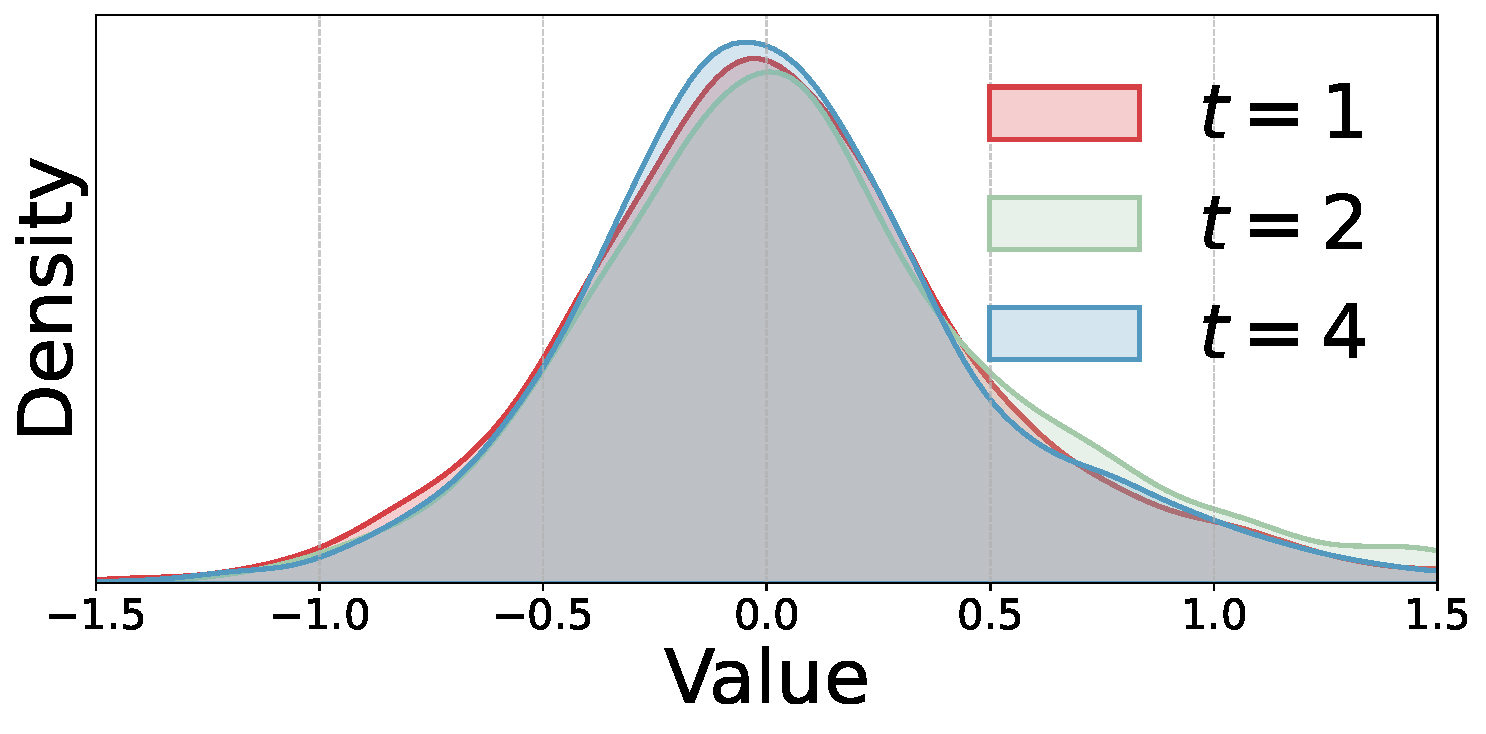
\includegraphics[width=0.95\linewidth]{fig/density_plot_presynaptic_input_mpinit.pdf}
    \caption{MP-Init}
  \end{subfigure}
  \caption{Activation distribution of the convolutional layer after the third layer's first spiking layer of ResNet-19 on CIFAR100}
  \label{fig:combined_activation}
\end{figure}

\subsection{Root Cause of TCS}\label{sec:root}

We first identify that TCS in activations fundamentally originates from TCS in membrane potentials. According to \cref{eq:lif_discrete_firing}, spike outputs depend directly on membrane potentials. If membrane potentials significantly drift over timesteps, the resulting activation distribution shifts correspondingly.

We empirically visualize the membrane potential at each timestep to validate this claim. As illustrated in \cref{fig:combined_membrane}, the membrane potential in tdBN, which does not account for the TCS problem, exhibits a clear temporal drift, leading to TCS in activation (\cref{fig:combined_activation}). While TEBN and TAB attempt to stabilize the distribution by timestep-dependent normalizations, the membrane potential itself continues to undergo transient drift, preserving TCS in activation.

\subsection{Convergence of Membrane Potential}
\label{sec:first_method_convergence}
While we have empirically demonstrated the existence of TCS in the membrane potential, a theoretical perspective can provide a deeper understanding. In this section, we present the core principles explaining why the membrane potential drifts over time.

We prove that the layer-wise distribution of membrane potential converges to a distribution possibly differing from its initial state as time progresses. This was proven on continuous-time LIF models with stable input statistics~\cite{dumont:2017}. Here, we extend this idea to the discrete-time model and show it has the same property. Let's start with the following assumption:

\textbf{Assumption 1.}
Assume $\{I_{\text{in}}[t]\}_{t\ge1}$ be a sequence drawn from an i.i.d. distribution. Furthermore, suppose there exist real constants $u^- < u^+$ where the membrane potential $U[t]$ of active neurons within each layer remains within $[u^-, u^+]$ for all $t$.

This i.i.d.\ assumption is reasonable, as inputs ${I_{\text{in}}[t]}_{t\ge1}$ are repeatedly drawn from a dataset or a normalized layer. Although soft reset LIF dynamics do not strictly prevent unbounded growth, well-trained SNNs rarely exhibit it in active neurons. The empirical validation of this assumption is provided in the supplementary material (\cref{subsec:validation_of_assumption_1}). Based on Assumption 1, we present the following theorem:

\textbf{Theorem 1.}
Under Assumption 1, the sequence $\{U[t]\}_{t \ge 0}$ forms a Markov chain with transition kernel $P$. This chain satisfies Doeblin’s minorization condition, ensuring the existence of a unique stationary distribution $\pi$. Moreover, the Total Variation (TV) distance between $U[t]$ and $\pi$ decreases exponentially.

Detailed proof is provided in supplementary material (\cref{subsec:proof_of_theorem_1}). This theorem indicates that TCS in the membrane potential is inevitable when the initial membrane potential differs from its stationary distribution. Traditionally, the membrane potential is initialized to zero, i.e., \(U[0] = 0\), but this zero initialization is a primary contributor to TCS. Therefore, to mitigate TCS, we must reduce the difference between the initial membrane potential and its stationary distribution.

\subsection{Membrane Potential Initialization}

Theorem 1 implies that eliminating the mismatch between the initial state and this stationary distribution is crucial. However, directly computing \(\pi\) is intractable; hence, we propose a more practical approach to initialize the membrane potential with a \textbf{per-layer constant} that approximates the mean of \( \pi \), as supported by the following lemma:

\textbf{Lemma 1.} Among all constants \( c \in \mathbb{R} \), \( c = E[\pi] \) minimizes expected square difference \(E[(\pi-c)^{2}]\).

The proof is provided in supplementary material (\cref{subsec:proof_of_lemma_1}). This lemma suggests that initializing the membrane potential to the mean of its stationary distribution is optimal for eliminating drift and minimizing variance. However, the next challenge lies in approximating \(E[\pi]\).

One simple solution is leveraging Theorem 1, which states that a membrane potential distribution exponentially converges to \(\pi\) over time. Therefore, we approximate \(\pi\) using the membrane potential at the final timestep (\(U[T]\)), which is the closest to \(\pi\). Based on this, we estimate the per-layer statistics of \(E[\pi]\) using \(E[U[T]]\).

To implement this efficiently, we compute the average membrane potential \(U[T]\) at the final timestep \(T\) for each layer during training. This average is then used to update a running mean \(r\), which is initialized to zero at the beginning of training. Before feeding each batch into the network (during both training and inference), we initialize the membrane potential of every layer to this running mean, i.e., \(U[0] = r\). This technique is called \textbf{MP-Init}, which requires minimal extra memory or computation.

As illustrated in \cref{fig:combined_membrane,fig:combined_activation}, MP-Init effectively resolves both TCS in membrane potential and activation, resulting in consistent distributions over time. Importantly, MP-Init is straightforward to implement and does not require modifications to BN layers or involve complex training pipelines, unlike methods such as TEBN~\cite{tebn:2022} or TAB~\cite{tab:2024}. This simplicity and ease of implementation significantly enhance the usability of SNNs across various applications without altering existing recipes. 
